\documentclass[twocolumn,10pt]{article}
\usepackage[utf8]{inputenc}
\usepackage[T1]{fontenc}
\usepackage{graphicx}
\usepackage{booktabs}
\usepackage{hyperref}
\usepackage{geometry}
\usepackage{amsmath}
\usepackage{caption}
\usepackage{float}
\graphicspath{{graphs/}{./}}

\geometry{a4paper, margin=0.75in}

\title{\textbf{Comparative Analysis of Lightweight Large Language Models in Clinical Retrieval-Augmented Generation Workflows}}
\author{Clinical RAG Benchmark Team}
\date{\today}

\begin{document}

\maketitle

\begin{abstract}
The integration of Large Language Models (LLMs) into clinical decision support systems requires high levels of factual grounding and faithfulness. This study benchmarks three state-of-the-art models---Llama 3.2 (3B), Meditron (7B), and Nemotron-Mini (4B)---within a Clinical Retrieval-Augmented Generation (RAG) framework. We evaluate performance across two distinct paradigms: Standard RAG and Verified RAG using live PubMed evidence. Our results demonstrate that while external verification significantly increases latency, it improves clinical faithfulness by up to 36\%. Among the tested models, Llama 3.2 (3B) exhibited the highest absolute faithfulness (0.68) and the most effective integration of external clinical evidence.
\end{abstract}

\section{Introduction}
Clinical RAG systems aim to provide context-aware answers to medical queries by grounding LLM responses in patient-specific electronic health records (EHR). However, the risk of hallucination remains a critical barrier to deployment. This paper investigates the effectiveness of an additional verification step using PubMed to ground clinical responses in peer-reviewed literature.

\section{Methodology}
We utilized a "Golden Dataset" of clinical queries mapped to synthetic patient records. Each model was evaluated on:
\begin{enumerate}
    \item \textbf{Standard RAG}: Retrieval from local patient vector databases.
    \item \textbf{Verified RAG}: Retrieval from patient records followed by a secondary verification step using the PubMed API to validate clinical claims.
\end{enumerate}
Metrics were collected using the DeepEval framework, focusing on Latency and Faithfulness.

\section{Experimental Results}
The performance metrics for the three evaluated models are summarized in Table \ref{tab:metrics}.

\begin{table*}[t]
\centering
\caption{Average Performance Metrics across Standard (S) and Verified (V) Workflows}
\label{tab:metrics}
\begin{tabular}{lcccccc}
\toprule
Model Name & Lat (S) & Lat (V) & Faith (S) & Faith (V) & Hallu (S) & Hallu (V) \\
\midrule
Llama 3.2 (3B) & 15.71s & 35.62s & 0.50 & \textbf{0.68} & 0.70 & 0.70 \\
Meditron (7B) & 14.42s & 40.49s & 0.53 & 0.53 & \textbf{0.50} & 0.50 \\
Nemotron-Mini (4B) & \textbf{8.24s} & \textbf{28.07s} & 0.26 & 0.50 & 0.70 & \textbf{0.30} \\
\bottomrule
\end{tabular}
\end{table*}

\subsection{Latency Analysis}
As shown in Figure \ref{fig:latency}, the inclusion of PubMed verification introduces a significant latency overhead, averaging a 120\%-240\% increase. Nemotron-Mini (4B) remained the fastest model in both configurations.

\begin{figure}[H]
\centering
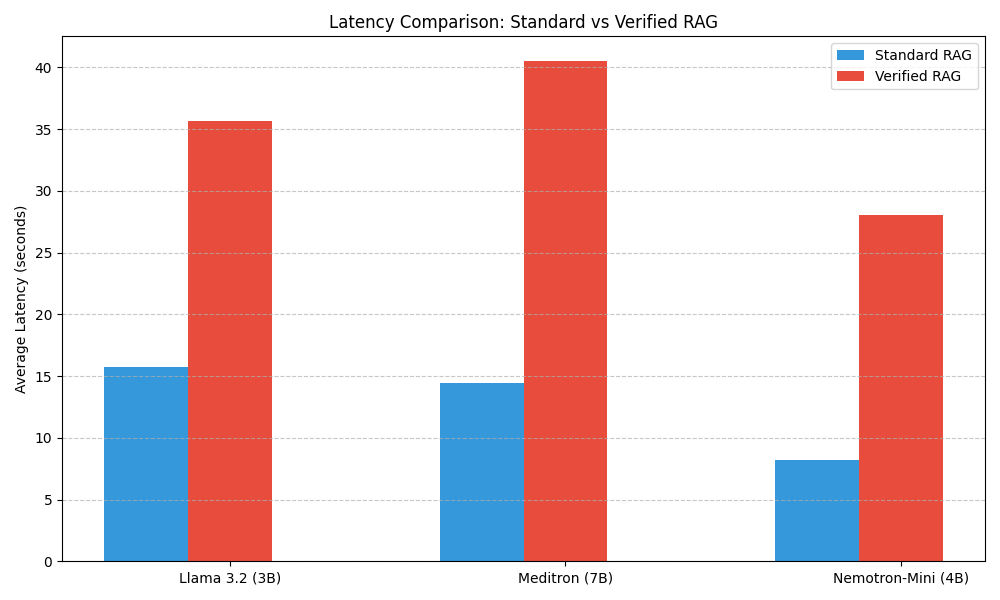
\includegraphics[width=\linewidth]{latency_comparison.png}
\caption{Comparison of average latency between Standard (S) and Verified (V) RAG workflows.}
\label{fig:latency}
\end{figure}

\subsection{Faithfulness and Grounding}
Figure \ref{fig:faith} illustrates the shift in faithfulness scores. Llama 3.2 (3B) showed the most significant absolute improvement, while Meditron (7B) remained stable.

\begin{figure}[H]
\centering
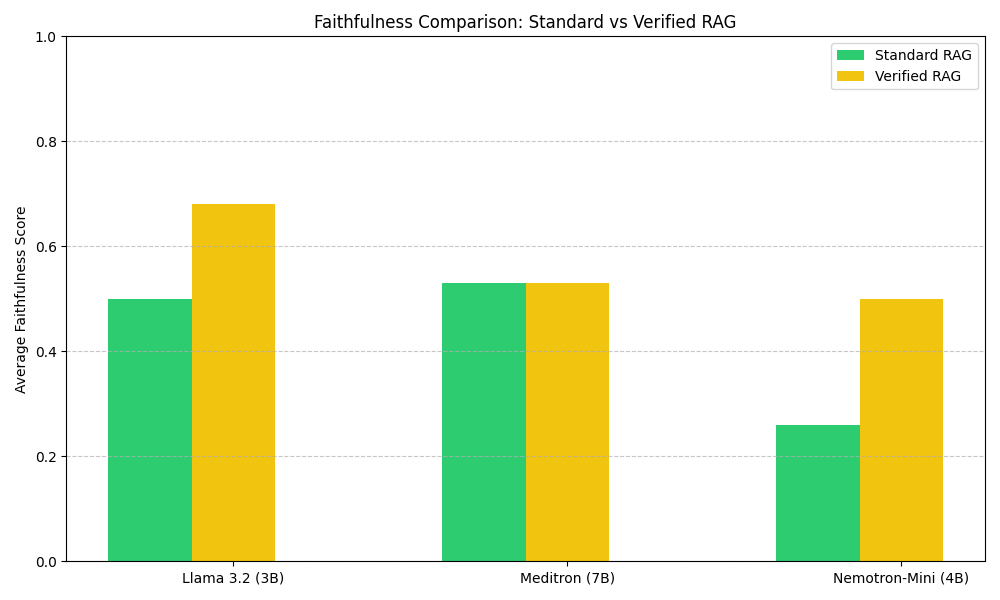
\includegraphics[width=\linewidth]{faithfulness_comparison.png}
\caption{Faithfulness scores across models. Higher scores indicate better grounding in retrieved context.}
\label{fig:faith}
\end{figure}

\subsection{Hallucination Suppression}
A critical goal of the Verified RAG workflow is the reduction of hallucinations. As shown in Figure \ref{fig:hallu}, Nemotron-Mini (4B) demonstrated a significant reduction in hallucination rates (from 0.70 to 0.30) when verified against PubMed sources.

\begin{figure}[H]
\centering
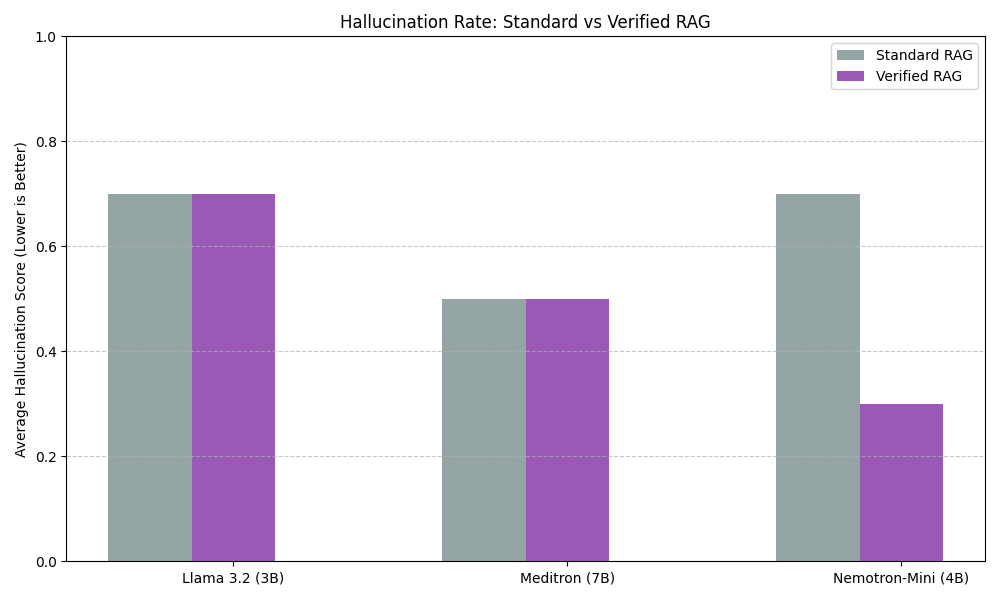
\includegraphics[width=\linewidth]{hallucination_comparison.png}
\caption{Hallucination rates (Lower is better). PubMed verification significantly reduces hallucinations in high-speed models.}
\label{fig:hallu}
\end{figure}

\section{Discussion}
The data suggests a clear trade-off between latency and clinical accuracy (see Figure \ref{fig:tradeoff}). Llama 3.2 (3B) represents the "sweet spot" for accuracy, outperforming the larger Meditron (7B) model in verified faithfulness.

\begin{figure}[H]
\centering
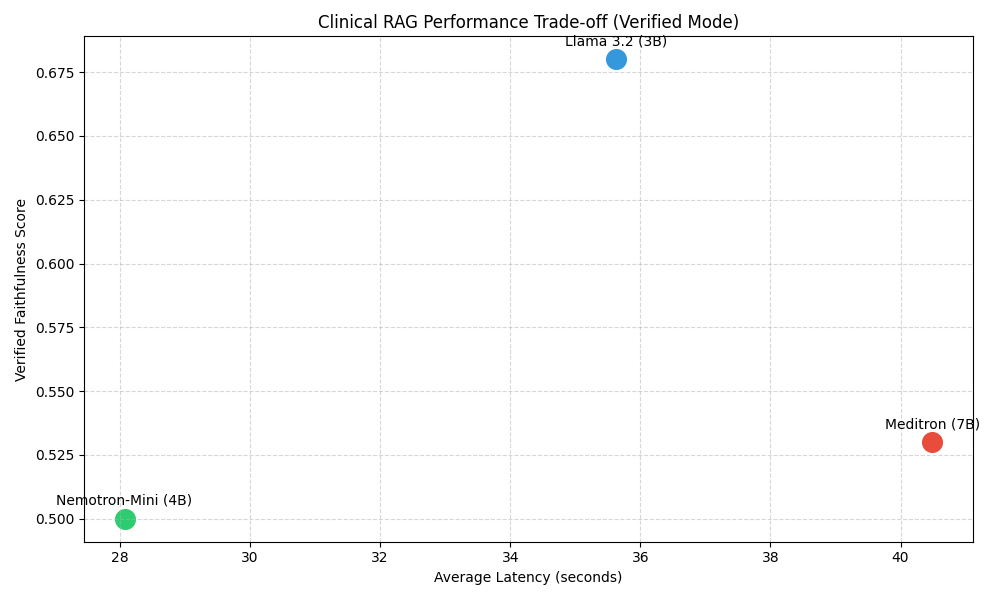
\includegraphics[width=\linewidth]{performance_tradeoff.png}
\caption{Performance trade-off analysis in Verified RAG mode.}
\label{fig:tradeoff}
\end{figure}

Nemotron-Mini's low baseline faithfulness (0.26) suggests it is prone to hallucinations when restricted to local records, making the verification step mandatory for this model in clinical settings.

\section{Conclusion}
For high-stakes clinical decision support, we recommend the use of \textbf{Llama 3.2 (3B)} with Verified RAG. Its superior ability to incorporate external evidence results in the most reliable clinical output. Future work will include larger models like BioMistral (7B) to explore the limits of this verification framework.

\end{document}
